% Whittle Laboratory Beamer Template
% Based on the University of Cambridge beamer remplate by Rich Wareman 
% J. Brind
% Sept 2018

%%%%%%%%%%%%%%%%%%%
% TEMPLATE SET UP %
%%%%%%%%%%%%%%%%%%%

% Use Beamer and the Cambridge theme
% option [unknownkeysallowed] is required to compile on my windows box 
\documentclass[unknownkeysallowed]{beamer}
\usetheme{cambridge}

% Required packages
\usepackage{appendixnumberbeamer} % New slide numbers for the appendix
\usepackage{helvet} % quasi-Arial font
\usepackage[T1]{fontenc} % proper hyphenation in foreign languages

% Optional packages
\usepackage{amssymb} % Extra maths symbols
\usepackage{siunitx} % Units

% Miscellaneous declarations
\setlength\fboxrule{1pt} % thick line around boxed text
\usefonttheme[onlymath]{serif} % equations in black
\sisetup{range-units=single} % only one unit in a numerical range
\sisetup{math-rm = \ensuremath} 
\setbeamercovered{transparent} % inactive text is semitransparent

% Define a command for absolute positioning
\def\Put(#1,#2)#3{\leavevmode\makebox(0,0){\put(#1,#2){#3}}}

% Define footer reference boxes
% Two-line
\usepackage[absolute,overlay]{textpos}
\newcommand{\footreftwo}[1]{%
 \begin{textblock*}{7.8cm}(2.75cm,8.54cm)%
    \vspace{0.05em}\flushleft%
    \colorlet{saved}{.}\color{white}%
    \tiny #1%
    \color{saved}%
 \end{textblock*}
}
% Three-line
\newcommand{\footrefthree}[1]{%
  \begin{textblock*}{7.8cm}(2.75cm,8.43cm)%
    \vspace{0.05em}\flushleft%
    \colorlet{saved}{.}\color{white}%
    \tiny #1%
    \color{saved}%
  \end{textblock*}
}

% Nomenclature macros 
\newcommand{\etal}{\emph{et al.\@} }
\newcommand{\BR}{\mathit{B\kern-.15em R}}
\newcommand{\IR}{\mathit{I\kern-.15emR}}
\newcommand{\DR}{\mathit{D\kern-.15emR}}
\newcommand{\PR}{\mathit{P\kern-.15emR}}
\newcommand{\Rey}{\mathit{Re}}
\newcommand*\df{\mathop{}\!\mathrm{d}}
\newcommand*\Df{\mathop{}\!\mathrm{D}}

%%%%%%%%%%%%%%%%%%%%%%%
% Author, Title, etc. %
%%%%%%%%%%%%%%%%%%%%%%%

\title{Example Presentation}

\author{\normalsize\textbf{James Brind, Graham Pullan} \\ 
Whittle Laboratory \\
University of Cambridge \\
Cambridge, CB3 0DY, UK \\
Email: jb753@cam.ac.uk}

\date{\normalsize\today}

%%%%%%%%%%%%%%%%%%%%%%%%% The main document %%%%%%%%%%%%%%%%%%%%%%%%%

\begin{document}

\begin{frame}
  \titlepage
\end{frame}

\begin{frame}{Example Figure}
  \centering
  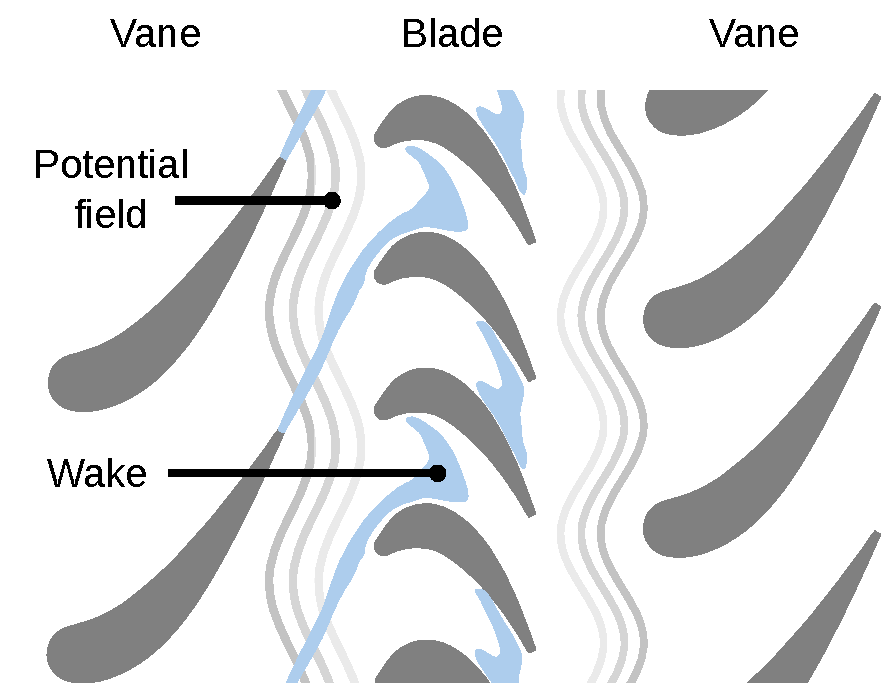
\includegraphics[width=0.9\linewidth,trim={0 1.5cm 0 0},clip]{figures/blade_row_interactions.pdf}
\end{frame}

\part{Example Part}
\frame{\partpage}

\begin{frame}{Itemize}
  \begin{itemize}
    \item item
    \item item
   \alert{\item alert}
  \end{itemize}
\end{frame}

\begin{frame}{Overlays}
  \begin{itemize}
    \item<1,4> item
    \item<2,4> item
    \item<3,4> item
  \end{itemize}
\end{frame}

\begin{frame}{Block environments}
  \begin{block}{Block}
    This is a block.\\
    A block with two lines.
  \end{block}
  \begin{exampleblock}{Example}
    This is an example.
  \end{exampleblock}

\end{frame}

\begin{frame}{Theorems}

  \begin{theorem}[Author]
    This is a theorem.\\
    \[ a^2 = b^2 + c^2\]
  \end{theorem}
  \begin{definition}
    This is a theorem.\\
    \[ a^2 = b^2 + c^2\]
  \end{definition}

\footrefthree{A three line reference. A three line reference. A three line reference. A three line reference. A three line reference. A three line reference. A three line reference. A three line reference. A three line reference. }


\end{frame}

\begin{frame}{Proof}

  \begin{proof}[My proof]
    This is a proof.\\
  \end{proof}

\footreftwo{A two line reference. A two line reference. A two line reference. A two line reference. A two line reference. A two line reference. A two line reference. }

\end{frame}

\begin{frame}{Columns}
  \dblcol{%
    Bottom
    \vfill
    Top
  }{%
    Centre
  }
\end{frame}


\end{document}


